\documentclass[twoside,11pt]{homework}

\coursename{COMS 4236: Computational Complexity (Fall 2018)} 

\studname{Wenbo Gao}    % YOUR NAME GOES HERE
\studmail{wg2313@columbia.edu}% YOUR UNI GOES HERE
\hwNo{1}                   % THE HOMEWORK NUMBER GOES HERE
\date{\today} % DATE GOES HERE

% Uncomment the next line if you want to use \includegraphics.
\usepackage{graphicx}
%\includegraphics[height=0.3\textheight]{hw0.pdf}
\usepackage{physics}
% \usepackage{tikz}

% \usetikzlibrary{fit,positioning,arrows,automata,calc}
% \tikzset{
%   main/.style={circle, minimum size = 15mm, thick, draw =black!80, node distance = 10mm},
%   connect/.style={-latex, thick},
%   box/.style={rectangle, minimum height = 8mm,draw=black!100}
% }

% environments: theorem[*rename], proof[*rename], 

\begin{document}
\maketitle

\section*{Problem 1}
(Problem 3.14 on page 149 of TC (8 points))
Show that the collection of decidable languages is closed under the operations
of
\textbf{a)} union.
\textbf{b)} concatenation. Given two languages $L$ and $L'$, their
concatenation is the following language $L^*$: a string $\mathbf{w} = w_1 \dots
w_2$ is in $L^*$ if there exists an $i$ such that $w_1 \dots w_i \in L$ and
$w_{i+1}\dots w_n \in L'$.
\textbf{c)} complementation.
\textbf{d)} intersection.

(Xi: I removed the operation of "star" from the problem but its solution is
similar to that of "concatenation".)

\subsection*{a) union}

\begin{solution}
  Let $\bbM$ be the set of all Turing machines and\\ $\bbL = \{ L : \forall L \in \Sigma^*, \exists M
  \in \bbM, L = L(M) \}$ be the set of all decidable languages.
  \[
    \begin{aligned}
      \forall L_1 \in \bbL, \exists M_1 \in \bbM, L_1 = L_1(M_1).\\
      \Rightarrow M_1(w) =
      \left\{
      \begin{aligned}
        1 ;& \text{ if } w \in L_1\\
        0 ;& \text{ if } w \in \Sigma^* / L_1
      \end{aligned}
      \right. \\
      \forall L_2 \in \bbL, \exists M_2 \in \bbM, L_2 = L_2(M_2).\\
      \Rightarrow M_2(w) =
      \left\{
      \begin{aligned}
        1 ;& \text{ if } w \in L_2\\
        0 ;& \text{ if } w \in \Sigma^* / L_2
      \end{aligned}
      \right. \\
    \end{aligned}
  \]

  Let $L = L_1 \cup L_2 = \{ w : \forall w \in \Sigma^*, w \in L_1 \lor w \in L_2\}$ be the union
  of $L_2$ and $L_2$.
  \begin{construct}[Turing machine $D$]
    \[
      D(w) =
      \left\{
        \begin{aligned}
          1 ; & \text{ if } M_1(w) = 1 \lor M_2(w) = 1\\
          0 ; & \text{ otherwise}
        \end{aligned}
      \right.
      =
      \left\{
        \begin{aligned}
          1 ; & \text{ if } w \in L_1 \lor w \in L_2\\
          0 ; & \text{ otherwise}
        \end{aligned}
      \right.
      =
      \left\{
        \begin{aligned}
          1 ; & \text{ if } w \in L\\
          0 ; & \text{ if } w \in \Sigma^* / L
        \end{aligned}
      \right.\\
    \]
  \end{construct}

  Thus, $L = L(D) \Rightarrow L \in \bbL \Rightarrow \bbL$ is closed under union.

\end{solution}

\subsection*{b) concatenation}

\begin{solution}
  Let $\bbM$ be the set of all Turing machines and\\ $\bbL = \{ L : \forall L \in \Sigma^*, \exists M
  \in \bbM, L = L(M) \}$ be the set of all decidable languages.
  \[
    \begin{aligned}
      \forall L_1 \in \bbL, \exists M_1 \in \bbM, L_1 = L_1(M_1).\\
      \forall L_2 \in \bbL, \exists M_2 \in \bbM, L_2 = L_2(M_2).\\
    \end{aligned}
  \]

  Let $L = \{ \mathbf{w} : \mathbf{w} = (w_1, \dots, w_n),
  \exists i \in \bbN, (w_1, \dots, w_i) \in L_1 \land (w_{i+1}, \dots, w_n) \in L_2 \}$ be
  the concatenation of $L_1$ and $L_2$.

  \begin{construct}[Turing machine $D$]
    \[
      \begin{aligned}
        D(w) =&\\
        &\text{let}\\
        &\quad n = |w| \text{, and initialize variable } b = 0 \text{ (false)}\\
        &\text{in}\\
        &\quad i \leftarrow [0, 1, 2, \dots, n] \text{ (try all possible break points)}\\
        &\quad\quad b = b \lor (M_1(w_1 \dots w_i) \land M_2(w_{i+1} \dots w_n))\\
        &\quad \text{return } b
      \end{aligned}
    \] 
  \end{construct}

  Thus, $L = L(D) \Rightarrow L \in \bbL \Rightarrow \bbL$ is closed under concatenation.

\end{solution}

\subsection*{c) complementation}

\begin{solution}
  Let $\bbM$ be the set of all Turing machines and\\ $\bbL = \{ L : \forall L \in \Sigma^*, \exists M
  \in \bbM, L = L(M) \}$ be the set of all decidable languages.
  \[
    \begin{aligned}
      \forall L_1 \in \bbL, \exists M_1 \in \bbM, L_1 = L_1(M_1).\\
      \Rightarrow M_1(w) =
      \left\{
      \begin{aligned}
        1 ;& \text{ if } w \in L_1\\
        0 ;& \text{ if } w \in \Sigma^* / L_1
      \end{aligned}
      \right. \\
    \end{aligned}
  \]

  Let $L = \Sigma^* / L_1$ be the complement set of $L_1$.

  \begin{construct}[Turing machine $D$]
    \[
      D(w) = \lnot M_1(w) =
      \left\{
      \begin{aligned}
        1 ;& \text{ if } w \in \Sigma^* / L_1\\
        0 ;& \text{ if } w \in L_1
      \end{aligned}
      \right.
      =
      \left\{
      \begin{aligned}
        1 ;& \text{ if } w \in L\\
        0 ;& \text{ if } w \in \Sigma^* / L
      \end{aligned}
      \right. 
    \]
  \end{construct}

  Thus, $L = L(D) \Rightarrow L \in \bbL \Rightarrow \bbL$ is closed under complement.

\end{solution}

\subsection*{d) intersection}

\begin{solution}
  Let $\bbM$ be the set of all Turing machines and\\ $\bbL = \{ L : \forall L \in \Sigma^*, \exists M
  \in \bbM, L = L(M) \}$ be the set of all decidable languages.
  \[
    \begin{aligned}
      \forall L_1 \in \bbL, \exists M_1 \in \bbM, L_1 = L_1(M_1).\\
      \Rightarrow M_1(w) =
      \left\{
      \begin{aligned}
        1 ;& \text{ if } w \in L_1\\
        0 ;& \text{ if } w \in \Sigma^* / L_1
      \end{aligned}
      \right. \\
      \forall L_2 \in \bbL, \exists M_2 \in \bbM, L_2 = L_2(M_2).\\
      \Rightarrow M_2(w) =
      \left\{
      \begin{aligned}
        1 ;& \text{ if } w \in L_2\\
        0 ;& \text{ if } w \in \Sigma^* / L_2
      \end{aligned}
      \right. \\
    \end{aligned}
  \]

  Let $L = L_1 \cap L_2 = \{ w : \forall w \in \Sigma^*, w \in L_1 \land w \in L_2\}$ be the intersection of $L_2$ and $L_2$.
  \begin{construct}[Turing machine $D$]
    \[
      D(w) =
      \left\{
        \begin{aligned}
          1 ; & \text{ if } M_1(w) = 1 \land M_2(w) = 1\\
          0 ; & \text{ otherwise}
        \end{aligned}
      \right.
      =
      \left\{
        \begin{aligned}
          1 ; & \text{ if } w \in L_1 \land w \in L_2\\
          0 ; & \text{ otherwise}
        \end{aligned}
      \right.
      =
      \left\{
        \begin{aligned}
          1 ; & \text{ if } w \in L\\
          0 ; & \text{ if } w \in \Sigma^* / L
        \end{aligned}
      \right.\\
    \]
  \end{construct}

  Thus, $L = L(D) \Rightarrow L \in \bbL \Rightarrow \bbL$ is closed under intersection.

\end{solution}

\section*{Problem 2}

(Problem 3.17 on page 149 of TC (10 points))*
Show that single-tape TMs that cannot write on the portion of the tape
containing the input string can only decide regular languages.

(Xi: A regular language is a language accepted by a finite-state automaton.
Given such a TM, what are the states of your automaton?
You will receive 7 points by solving Problem 3.13, an easier version of 3.17.)

\begin{solution}
  First, let's consider read-only TMs with no access to cells outside input cells.\\
  A read-only TM with its pointer only moving right, $M_1$, is strictly a
  finite-state automaton (FSA).\\
  A read-only TM with its pointer moving left and right, $M_2$, is equivalent to
  $M_1$ with a longer input tape which contains the entire path of $M_2$'s
  pointer from start to halt. (Figure \ref{fig:01})

  \begin{figure}[h]
  	\centering
  	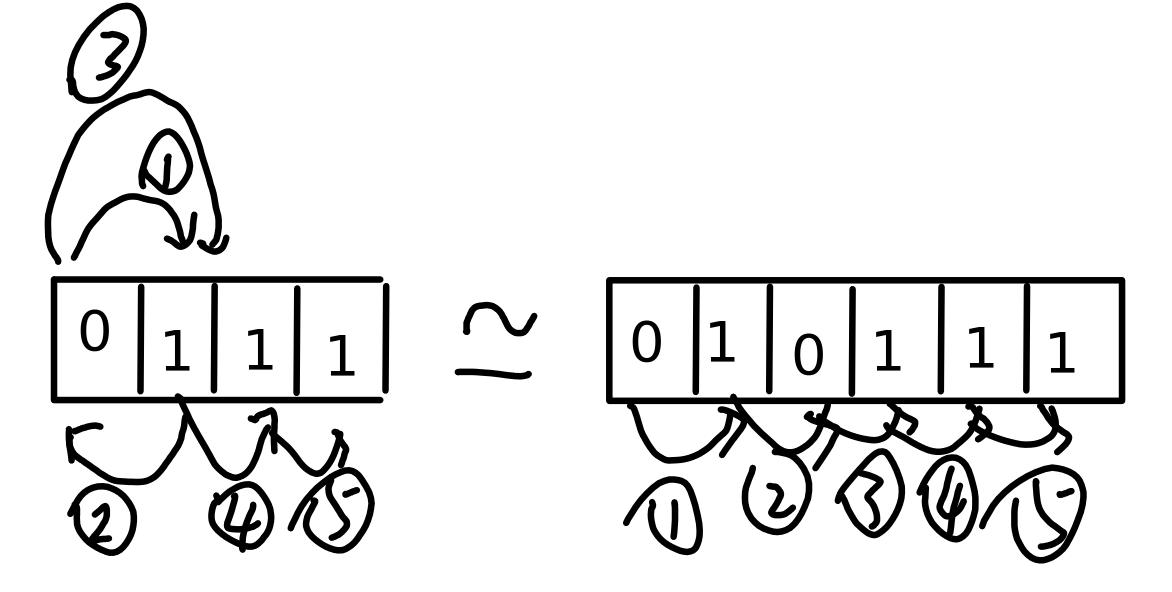
\includegraphics[width=0.7\linewidth]{img/01.png}
  	\caption{an example}
  	\label{fig:01}
  \end{figure}

  If the read-only TMs access the empty cells outside input cells,
  there are three new possible termination cases:
  \begin{enumerate}
  \item halt inside input cells
  \item halt outside input cells
  \item run forever.
  \end{enumerate}

  The third case doesn't add to the accepted inputs which can be ignored.\\
  For the first two, since operations on empty cells won't add any information to
  the system but sorely rely on the FSA part of the TM, we can merge the state
  transitions when pointer is outside input cells to the transitions inside the
  input cells: Figure \ref{fig:02}
  \begin{figure}[h]
  	\centering
  	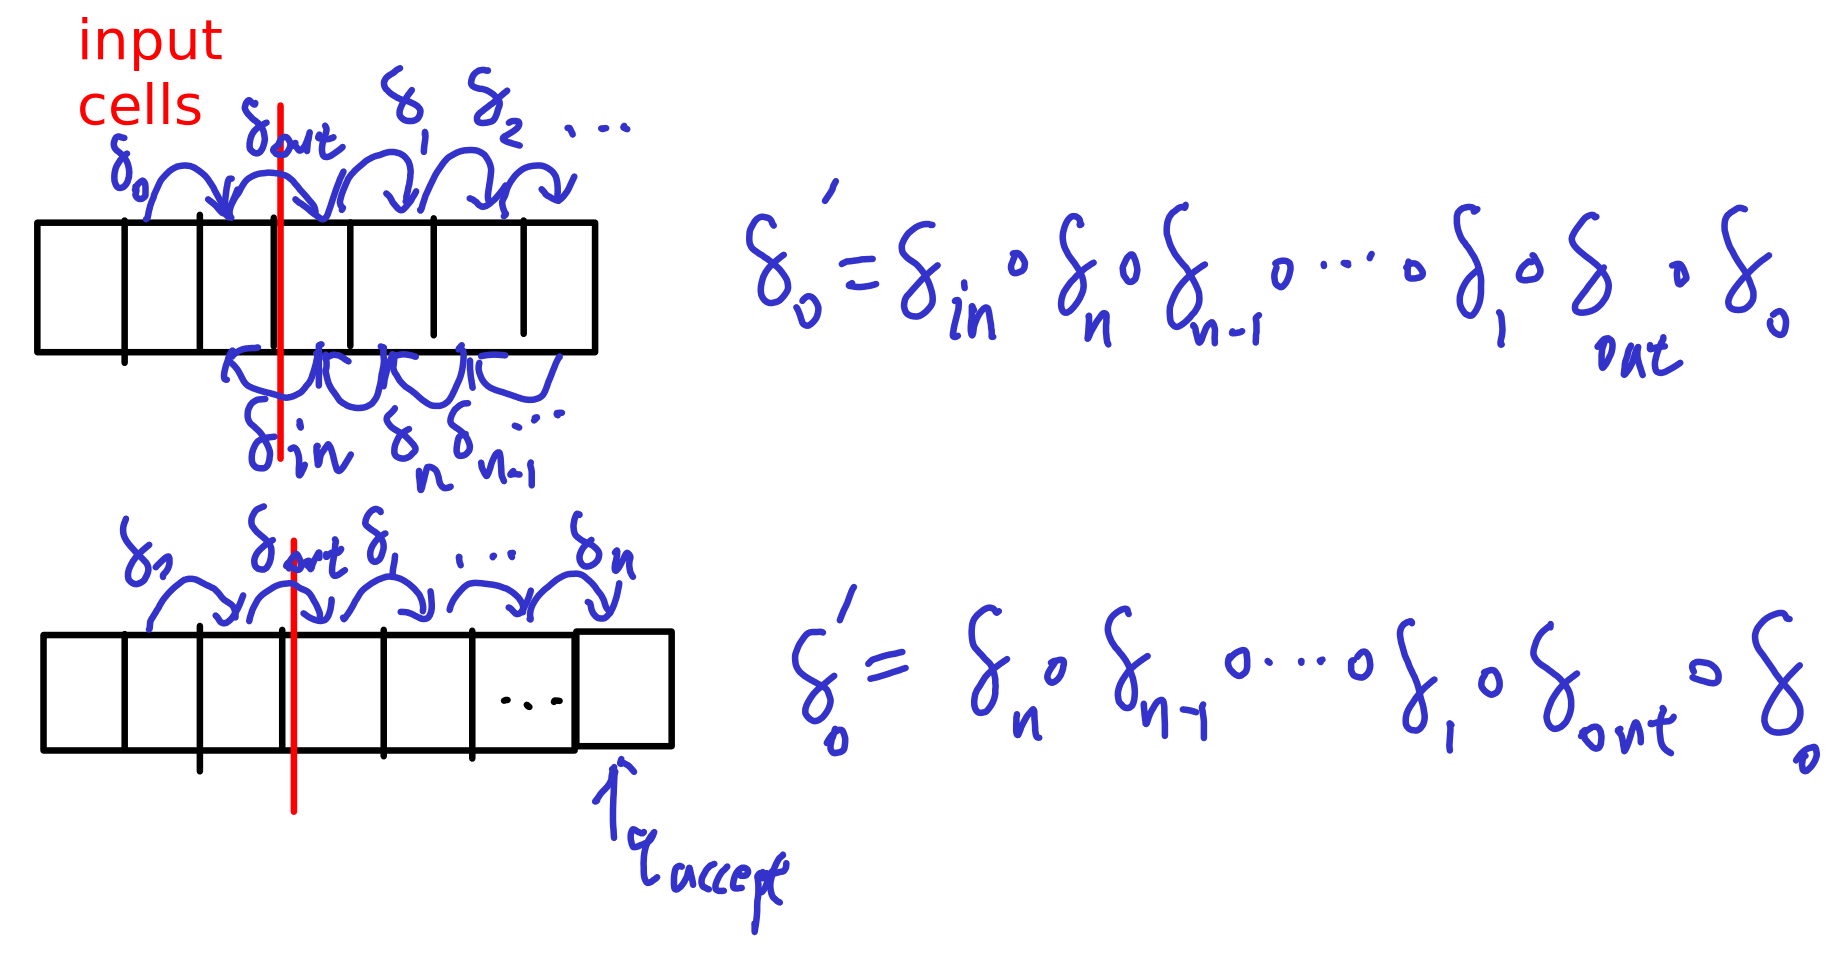
\includegraphics[width=0.7\linewidth]{img/02.png}
  	\caption{upper: the pointer moves back to input cells; lower: case 2 where
      the TM halts outside input cells.}
  	\label{fig:02}
  \end{figure}

  Thus, whether the read-only TMs access the empty cells or not, they are
  equivalent to FSAs, thus they can only decide regular languages.

\end{solution}

\section*{Problem 3}

(Problem 3.4.1 on page 66 of CC (12 points))
For each of the following problem involving Turing machines, determine whether
or not it is decidable:
\textbf{a)} Given a Turing machine $M$, does it halt on the empty string?
\textbf{b)} Given a Turing machine $M$, is there a string which it halts?
\textbf{c)} Given a Turing machine $M$, is $L(M)$ finite?
( Here $L(M)$ denotes the set of strings $\mathbf{w}$ which $M(\mathbf{w})$="yes".)
\textbf{d)} Given two Turing machines $M$ and $M'$, is $L(M) = L(M')$?
( Xi: To prove a problem is decidable, show that if there is a TM that decides
it, then one can construct a TM to decide the halting problem or\textit{a
  problem that you have already shown to be undecidable}. )

\subsection*{a) EmptyHalt}

\begin{solution}
  Let $\bbM$ be the set of all Turing machines. \\
  \[
    \begin{aligned}
      \text{Halt} &= \{ <M, w>: \forall M \in \bbM, \forall w \in \Sigma^*, M(w) = 1\}\\
      \text{EmptyHalt} &= \{ <M> : \forall M \in \bbM, M(\epsilon) = 1 \}
    \end{aligned}
  \]

  reduction from EmptyHalt to Halt:
  \begin{given}
    $<M ,w>$, where $M \in \bbM$ and $w \in \Sigma^*$
  \end{given}
  \begin{construct}[Turing machine $M'$ from $M$ with $w$ encoded in its FSA]
    $\forall \text{ input } w' \in \Sigma^*$,
    \begin{enumerate}
    \item erase input $w'$ from the tape
    \item write $w$ to the tape
    \item reset pointer to the beginning of the tape and reset state to $q_{start}$
    \item simulate $M$ on $w$
    \end{enumerate}
  \end{construct}
  Therefore, $\exists M' \in \bbM, \forall w' \in \Sigma^*, M'(w') = M(w)$ and thus $ M'(\epsilon) = M(w)$.\\
  If EmptyHalt is decidable then Halt is decidable.
  But Halt is not decidable so EmptyHalt is not decidable.

\end{solution}

\subsection*{b) Exist}
  Let $\bbM$ be the set of all Turing machines. \\
  \[
    \begin{aligned}
      \text{Halt} &= \{ <M, w>: \forall M \in \bbM, \forall w \in \Sigma^*, M(w) = 1\}\\
      \text{Exist} &= \{ <M> : \forall M \in \bbM, \exists w \in \Sigma^*, M(w) = 1 \}
    \end{aligned}
  \]

  \begin{given}
    $<M ,w>$, where $M \in \bbM$ and $w \in \Sigma^*$
  \end{given}
  Using the same construct as in \textbf{a)},
  we have $\exists M' \in \bbM, \forall w' \in \Sigma^*, M'(w') = M(w)$.\\
  If Exist is decidable then Halt is decidable.
  But Halt is not decidable so Exist is not decidable.

\subsection*{c) Finite}
  Let $\bbM$ be the set of all Turing machines. \\
  \[
    \begin{aligned}
      \text{Halt} &= \{ <M, w>: \forall M \in \bbM, \forall w \in \Sigma^*, M(w) = 1\}\\
      \text{Finite} &= \{ <M> : \forall M \in \bbM, L(M) \text{ is finite} \}
    \end{aligned}
  \]
  \begin{given}
    $<M ,w>$, where $M \in \bbM$ and $w \in \Sigma^*$
  \end{given}
  Using the same construct as in \textbf{a)} but with its answer flipped, we have\\
  \[
    \exists M' \in \bbM, \forall w' \in \Sigma^*, M'(w') = \lnot M(w)
  \]
  Therefore, $M(w) = 1 \iff L(M') = \emptyset$ (which is finite).
  If Finite is decidable then Halt is decidable.
  But Halt is not decidable so Finite is not decidable.

\subsection*{d) Equal}
  Let $\bbM$ be the set of all Turing machines. \\
  \[
    \begin{aligned}
      \text{Halt} &= \{ <M, w>: \forall M \in \bbM, \forall w \in \Sigma^*, M(w) = 1\}\\
      \text{Equal} &= \{ <M_1, M_2> : \forall M_1 \in \bbM, \forall M_2 \in \bbM, L(M_1)=L(M_2) \}
    \end{aligned}
  \]

  reduction from Equal to Halt:
  \begin{given}
    $<M ,w>$, where $M \in \bbM$ and $w \in \Sigma^*$
  \end{given}
  \begin{construct}[Turing machine $M_1$ and $M_2$]
    \[
      M_1(w_1) =
      \left\{
        \begin{aligned}
          1 ; &\text{ if } w_1 = \epsilon\\
          0 ; &\text{ otherwise}
        \end{aligned}
      \right.
    \]
    \[
      M_2(w_2) =
      \left\{
        \begin{aligned}
          M(w) ;& \text{ if } w_2 = \epsilon\\
          0 ;& \text{ otherwise}
        \end{aligned}
      \right.
    \]
  \end{construct}
  Therefore, $M(w) = 1 \iff L(M_1) = L(M_2)$.\\
  If Equal is decidable then Halt is decidable.
  But Halt is not decidable so Equal is not decidable.

  



\section*{Problem 4}
(Problem 3.4.5 on page 67 of CC (10 points))
Show that $L$ is recursive if and only if there is a Turing machine $M$ that
enumerates $L$, and such that the strings in $L$ are output by $M$ in
length-increasing fashion.
(For the if direction, if $L$ is finite there is nothing to prove.
So suppose it is infinite.)
(Xi: Read pages 61-62 of CC or pages 140-141 of TC for the direction of a Turing
machine enumerating a language $L$.)

\subsection*{1) $ \forall L \subset \Sigma^*, \exists M \in \bbM, L = L(M) \Rightarrow \exists M' \in \bbM, L = E(M')$}

\begin{proof}
  \begin{given}
    \begin{enumerate}
    \item $L \subset \Sigma^*$
    \item $M \in \bbM$ such that $L = L(M)$
    \end{enumerate}
  \end{given}

  \begin{construct}[Turing machine $M'$ that enumerates $L$]
    $\forall \text{ input } x \in \Sigma^*$, \\
    enumerate $\Sigma^*$ ($w \leftarrow \Sigma^*$) in lexicographical order ($0, 1, 10, 11, 100, \dots$):
    \begin{enumerate}
    \item simulate $M$ on $w$, if $M(w) = 1$ then output $\sqcup w \sqcup$ at the end of
      the tape
    \item if $w = x$, then accept.
    \end{enumerate}
    
  \end{construct}
\end{proof}

\subsection*{2) $\forall L \subset \Sigma^*, \exists M \in \bbM, L = E(M) \Rightarrow \exists M' \in \bbM, L = L(M')$}

\begin{proof}
  \begin{given}
    \begin{enumerate}
    \item $L \subset \Sigma^*$
    \item $M \in \bbM$ such that $L = E(M)$
    \end{enumerate}
  \end{given}

  \begin{construct}[Turing machine $M'$ that determines $L$]
    $\forall \text{ input } x \in \Sigma^*$, \\
    simulate $M$ on $\epsilon$
    \begin{enumerate}
    \item if the tape ends with $\sqcup x \sqcup$, then accept.
    \item if the tape ends with $\sqcup w \sqcup$ where $|w| > |x|$, then reject.
    \end{enumerate}
    
  \end{construct}
\end{proof}

\end{document} 
